\documentclass[12pt]{article}
\usepackage[utf8]{inputenc}
\usepackage[utf8]{inputenc}
\usepackage{amsmath}
\usepackage{amsthm}
\usepackage{geometry}
\usepackage{amsfonts}
\usepackage{mathrsfs}
\usepackage{bm}
\usepackage{hyperref}
\usepackage[dvipsnames]{xcolor}
\usepackage[inline]{enumitem}
\usepackage{mathtools}
\usepackage{changepage}
\usepackage{lipsum}
\usepackage{tikz}
\usetikzlibrary{matrix, patterns}
\usepackage{tikz-cd}
\usepackage[nameinlink]{cleveref}
\geometry{
headheight=15pt,
left=60pt,
right=60pt
}
\setlength{\emergencystretch}{20pt}
\usepackage{fancyhdr}
\pagestyle{fancy}
\fancyhf{}
\lhead{}
\chead{Section 2.8 Exercises}
\rhead{\thepage}
\hypersetup{
    colorlinks=true,
    linkcolor=blue,
    urlcolor=blue
}

\theoremstyle{definition}
\newtheorem*{remark}{Remark}

\newtheoremstyle{exercise}
    {}
    {}
    {}
    {}
    {\bfseries}
    {.}
    { }
    {\thmname{#1}\thmnumber{#2}\thmnote{ (#3)}}
\theoremstyle{exercise}
\newtheorem{exercise}{Exercise 2.8.}

\newtheoremstyle{solution}
    {}
    {}
    {}
    {}
    {\itshape\color{magenta}}
    {.}
    { }
    {\thmname{#1}\thmnote{ #3}}
\theoremstyle{solution}
\newtheorem*{solution}{Solution}

\Crefformat{exercise}{#2Exercise 2.8.#1#3}

\newcommand{\ts}{\textsuperscript}
\newcommand{\setcomp}[1]{#1^{\mathsf{c}}}
\newcommand{\N}{\mathbf{N}}
\newcommand{\Z}{\mathbf{Z}}
\newcommand{\Q}{\mathbf{Q}}
\newcommand{\R}{\mathbf{R}}
\newcommand{\C}{\mathbf{C}}

\DeclarePairedDelimiter\abs{\lvert}{\rvert}
% Swap the definition of \abs* and \norm*, so that \abs
% and \norm resizes the size of the brackets, and the 
% starred version does not.
\makeatletter
\let\oldabs\abs
\def\abs{\@ifstar{\oldabs}{\oldabs*}}
%
\let\oldnorm\norm
\def\norm{\@ifstar{\oldnorm}{\oldnorm*}}
\makeatother

\setlist[enumerate,1]{label={(\alph*)}}

\begin{document}

\section{Section 2.8 Exercises}

Exercises with solutions from Section 2.8 of \hyperlink{ua}{[UA]}.

\begin{exercise}
\label{ex:1}
    Using the particular array \( (a_{ij}) \) from Section 2.1, compute \( \lim_{n \to \infty} s_{nn} \). How does this value compare to the two iterated values for the sum already computed?
\end{exercise}

\begin{solution}
    The array in question is
    \[
        \begin{bmatrix}
            -1 & \tfrac{1}{2} & \tfrac{1}{4} & \tfrac{1}{8} & \tfrac{1}{16} & \cdots \\[3mm]
            0 & -1 & \tfrac{1}{2} & \tfrac{1}{4} & \tfrac{1}{8} & \cdots \\[3mm]
            0 & 0 & -1 & \tfrac{1}{2} & \tfrac{1}{4} & \cdots \\[3mm]
            0 & 0 & 0 & -1 & \tfrac{1}{2} & \cdots \\[3mm]
            0 & 0 & 0 & 0 & -1 & \cdots \\[1mm]
            \vdots & \vdots & \vdots & \vdots & \vdots & \ddots
        \end{bmatrix},
    \]
    where \( a_{ij} = 1 / 2^{j-i} \) if \( j > i, a_{ij} = -1 \) if \( j = i \), and \( a_{ij} = 0 \) if \( j < i \). If we let \( f(j) \) be the sum of the first row up to the \( j \)\ts{th} column, then using the formula for the partial sums of a geometric series, we find that
    \begin{align*}
        f(j) &= \begin{cases}
            -1 & \text{if } j = 1, \\
            -1 + \tfrac{1}{2} + \cdots + \tfrac{1}{2^{j-1}} = -\tfrac{1}{2^{j-1}} & \text{if } j \geq 2
        \end{cases} \\[2mm]
        &= -\frac{1}{2^{j-1}}.
    \end{align*}
    Since subsequent rows are simply the first row shifted along, it is clear that \( s_{11} = f(1), s_{22} = f(1) + f(2), s_{33} = f(1) + f(2) + f(3) \), and in general
    \[
        s_{nn} = \sum_{j=1}^n f(j) = \sum_{j=1}^n \frac{-1}{2^{j-1}} = -\sum_{j=0}^{n-1} \frac{1}{2^j}.
    \]
    It follows that
    \[
        \lim_{n \to \infty} s_{nn} = -\sum_{j=0}^{\infty} \frac{1}{2^j} = -2.
    \]
    At the beginning of Section 2.1, we found that summing along the rows first gave a value for the double sum of \( 0 \), whereas summing down the columns first gave a value of \( -2 \).
\end{solution}

\begin{exercise}
\label{ex:2}
    Show that if the iterated series
    \[
        \sum_{i=1}^{\infty} \sum_{j=1}^{\infty} \abs{a_{ij}}
    \]
    converges (meaning for each fixed \( i \in \N \) the series \( \sum_{j=1}^{\infty} \abs{a_{ij}} \) converges to some real number \( b_i \), and the series \( \sum_{i=1}^{\infty} b_i \) converges as well), then the iterated series
    \[
        \sum_{i=1}^{\infty} \sum_{j=1}^{\infty} a_{ij}
    \]
    converges.
\end{exercise}

\begin{solution}
    For each \( i \in \N \), Theorem 2.7.6 implies that the series \( \sum_{j=1}^{\infty} a_{ij} \) converges to some real number \( c_i \). Observe that
    \[
        0 \leq \abs{c_i} = \abs{\sum_{j=1}^{\infty} a_{ij}} \leq \sum_{j=1}^{\infty} \abs{a_{ij}} = b_i.
    \]
    Since \( \sum_{i=1}^{\infty} b_i \) converges, the Comparison Test implies that the series \( \sum_{i=1}^{\infty} c_i \) is absolutely convergent and hence convergent.
\end{solution}

\begin{exercise}
\label{ex:3}
    \begin{enumerate}
        \item Prove that \( (t_{nn}) \) converges.

        \item Now, use the fact that \( (t_{nn}) \) is a Cauchy sequence to argue that \( (s_{nn}) \) converges.
    \end{enumerate}
\end{exercise}

\begin{solution}
    \begin{enumerate}
        \item Since \( \abs{a_{ij}} \geq 0 \) for all positive integers \( i \) and \( j \), the sequence \( (t_{nn}) \) is increasing and bounded above by the real number \( \sum_{i=1}^{\infty} \sum_{j=1}^{\infty} \abs{a_{ij}} \). Hence by the Monotone Convergence Theorem, \( (t_{nn}) \) converges.

        \item Suppose \( n > m \) are positive integers. By examining the array
        \[
            \begin{bmatrix}
                a_{11} & \cdots & a_{1m} & \cdots & a_{1n} \\
                \vdots & \ddots & \vdots & \ddots & \vdots \\
                a_{m1} & \cdots & a_{mm} & \cdots & a_{mn} \\
                \vdots & \ddots & \vdots & \ddots & \vdots \\
                a_{n1} & \cdots & a_{nm} & \cdots & a_{nn}
            \end{bmatrix},
        \]
        we see that
        \[
            \sum_{i=1}^n \sum_{j=1}^n a_{ij} - \sum_{i=1}^m \sum_{j=1}^m a_{ij} = \sum_{i=1}^m \sum_{j=m+1}^n a_{ij} + \sum_{i=m+1}^n \sum_{j=1}^n a_{ij}.
        \]
        (The sum of the top right ``square'' and the bottom ``rectangle'' of the array.) Let \( \epsilon > 0 \) be given. Since \( (t_{nn}) \) is a Cauchy sequence, there exists an \( N \in \N \) such that \( n > m \geq N \) implies that
        \[
            \abs{t_{nn} - t_{mm}} = t_{nn} - t_{mm} < \epsilon.
        \]
        For such \( n \) and \( m \), observe that
        \begin{align*}
            \abs{s_{nn} - s_{mm}} &= \abs{\sum_{i=1}^n \sum_{j=1}^n a_{ij} - \sum_{i=1}^m \sum_{j=1}^m a_{ij}} \\
            &= \abs{\sum_{i=1}^m \sum_{j=m+1}^n a_{ij} + \sum_{i=m+1}^n \sum_{j=1}^n a_{ij}} \\
            &\leq \sum_{i=1}^m \sum_{j=m+1}^n \abs{a_{ij}} + \sum_{i=m+1}^n \sum_{j=1}^n \abs{a_{ij}} \\
            &= t_{nn} - t_{mm} \\
            &< \epsilon.
        \end{align*}
        It follows that \( (s_{nn}) \) is a Cauchy sequence and hence convergent.
    \end{enumerate}
\end{solution}

\begin{exercise}
\label{ex:4}
    \begin{enumerate}
        \item Let \( \epsilon > 0 \) be arbitrary and argue that there exists an \( N_1 \in \N \) such that \( m, n \geq N_1 \) implies \( B - \tfrac{\epsilon}{2} < t_{mn} \leq B \).

        \item Now, show that there exists an \( N \) such that
        \[
            \abs{s_{mn} - S} < \epsilon
        \]
        for all \( m, n \geq N \).
    \end{enumerate}
\end{exercise}

\begin{solution}
    \begin{enumerate}
        \item By the approximation property for suprema, there exist positive integers \( m', n' \) such that \( B - \tfrac{\epsilon}{2} < t_{m' n'} \leq B \). Set \( N_1 = \max \{ m', n' \} \). Since each \( \abs{a_{ij}} \) is positive, \( (t_{mn}) \) is increasing in both \( m \) and \( n \); it follows that for \( m, n \geq N_1 \) we have \( B - \tfrac{\epsilon}{2} < t_{mn} \leq B \).

        \item Since \( \lim_{n \to \infty} s_{nn} = S \), there is an \( N_2 \in \N \) such that \( n \geq N_2 \) implies that \( \abs{s_{nn} - S} < \frac{\epsilon}{2} \). Set \( N = \max \{ N_1, N_2 \} \) and suppose that \( m, n > N \). Similarly to \Cref{ex:3} (b), we have
        \begin{align*}
            \abs{s_{mn} - s_{NN}} &= \abs{\sum_{i=1}^m \sum_{j=1}^n a_{ij} - \sum_{i=1}^N \sum_{j=1}^N a_{ij}} \\
            &= \abs{\sum_{i=1}^N \sum_{j=N+1}^n a_{ij} + \sum_{i=N+1}^m \sum_{j=1}^n a_{ij}} \\
            &\leq \sum_{i=1}^N \sum_{j=N+1}^n \abs{a_{ij}} + \sum_{i=N+1}^m \sum_{j=1}^n \abs{a_{ij}} \\
            &= t_{mn} - t_{NN} \\
            &\leq B - t_{NN} \\
            &< \tfrac{\epsilon}{2}.
        \end{align*}
        It follows that
        \[
            \abs{s_{mn} - S} \leq \abs{s_{mn} - s_{NN}} + \abs{s_{NN} - S} < \tfrac{\epsilon}{2} + \tfrac{\epsilon}{2} = \epsilon.
        \]
    \end{enumerate}
\end{solution}

\begin{exercise}
\label{ex:5}
    \begin{enumerate}
        \item Show that for all \( m \geq N \)
        \[
            \abs{(r_1 + r_2 + \cdots + r_m) - S} \leq \epsilon.
        \]
        Conclude that the iterated sum \( \sum_{i=1}^{\infty} \sum_{j=1}^{\infty} a_{ij} \) converges to \( S \).

        \item Finish the proof by showing that the other iterated sum, \( \sum_{j=1}^{\infty} \sum_{i=1}^{\infty} a_{ij} \), converges to \( S \) as well. Notice that the same argument can be used once it is established that, for each fixed column \( j \), the sum \( \sum_{i=1}^{\infty} a_{ij} \) converges to some real number \( c_j \).
    \end{enumerate}
\end{exercise}

\begin{solution}
    \begin{enumerate}
        \item Suppose that \( n \geq N \). Then
        \begin{align*}
            \abs{(r_1 + r_2 + \cdots + r_m) - S} &\leq \abs{(r_1 + r_2 + \cdots + r_m) - s_{mn}} + \abs{s_{mn} - S} \\
            &< \abs{(r_1 + r_2 + \cdots + r_m) - \left( \sum_{j=1}^n a_{1j} + \sum_{j=1}^n a_{2j} + \cdots + \sum_{j=1}^n a_{mj} \right)} + \epsilon \\
            &\leq \abs{r_1 - \sum_{j=1}^n a_{1j}} + \abs{r_2 - \sum_{j=1}^n a_{2j}} + \cdots + \abs{r_m - \sum_{j=1}^n a_{mj}} + \epsilon.
        \end{align*}
        Since this is true for any \( n \geq N \) and for any given \( i \) we have \( \sum_{j=1}^{\infty} a_{ij} = r_i \), taking the limit in \( n \) on both sides of the inequality
        \[
            \abs{(r_1 + r_2 + \cdots + r_m) - S} < \abs{r_1 - \sum_{j=1}^n a_{1j}} + \abs{r_2 - \sum_{j=1}^n a_{2j}} + \cdots + \abs{r_m - \sum_{j=1}^n a_{mj}} + \epsilon
        \]
        gives us
        \[
            \abs{(r_1 + r_2 + \cdots + r_m) - S} \leq \epsilon.
        \]
        It follows that \( \lim_{m \to \infty} \left( \sum_{i=1}^m r_i \right) = S \), i.e.\ \( \sum_{i=1}^{\infty} \sum_{j=1}^{\infty} a_{ij} = S \).

        \item Fix \( j \in \N \) and let \( (x_n) \) be the sequence of partial sums of the series \( \sum_{i=1}^{\infty} \abs{a_{ij}} \), i.e.\
        \[
            x_n = \abs{a_{1j}} + \abs{a_{2j}} + \cdots + \abs{a_{nj}}.
        \]
        Since each \( \abs{a_{ij}} \) is a term of the convergent series \( \sum_{j=1}^{\infty} \abs{a_{ij}} = r_i \), which has only non-negative terms, we see that \( \abs{a_{ij}} \leq r_i \), so that
        \[
            x_n \leq r_1 + r_2 + \cdots + r_n \leq \sum_{i=1}^{\infty} r_i,
        \]
        where the last inequality follows since each \( r_i \) is non-negative. So \( (x_n) \) is an increasing and bounded sequence and hence converges by the Monotone Convergence Theorem. It follows that \( \sum_{i=1}^{\infty} a_{ij} \) converges to some (non-negative) real number \( c_j \).

        Let \( \epsilon > 0 \) be given. As in \Cref{ex:4}, there is an \( N \in \N \) such that \( \abs{s_{mn} - S} < \epsilon \) for all \( m, n \geq N \). We can write \( s_{mn} \) as
        \[
            s_{mn} = \sum_{i=1}^m a_{i1} + \sum_{i=1}^m a_{i2} + \cdots + \sum_{i=1}^m a_{in}.
        \]
        Suppose that \( m, n \geq N \). Then
        \begin{align*}
            \abs{(c_1 + c_2 + \cdots + c_n) - S} &\leq \abs{(c_1 + c_2 + \cdots + c_n) - s_{mn}} + \abs{s_{mn} - S} \\
            &< \abs{(c_1 + c_2 + \cdots + c_n) - \left( \sum_{i=1}^m a_{i1} + \sum_{i=1}^m a_{i2} + \cdots + \sum_{i=1}^m a_{in} \right)} + \epsilon \\
            &\leq \abs{c_1 - \sum_{i=1}^m a_{i1}} + \abs{c_2 - \sum_{i=1}^m a_{i2}} + \cdots + \abs{c_n - \sum_{i=1}^m a_{in}} + \epsilon.
        \end{align*}
        Since this is true for any \( m \geq N \) and for any given \( j \) we have \( \sum_{i=1}^{\infty} a_{ij} = c_j \), taking the limit in \( m \) on both sides of the inequality
        \[
            \abs{(c_1 + c_2 + \cdots + c_n) - S} < \abs{c_1 - \sum_{i=1}^m a_{i1}} + \abs{c_2 - \sum_{i=1}^m a_{i2}} + \cdots + \abs{c_n - \sum_{i=1}^m a_{in}} + \epsilon
        \]
        gives us
        \[
            \abs{(c_1 + c_2 + \cdots + c_n) - S} \leq \epsilon.
        \]
        It follows that \( \lim_{n \to \infty} \left( \sum_{j=1}^n c_j \right) = S \), i.e.\ \( \sum_{j=1}^{\infty} \sum_{i=1}^{\infty} a_{ij} = S \).
    \end{enumerate}
\end{solution}

\begin{exercise}
\label{ex:6}
    \begin{enumerate}
        \item Assuming the hypothesis---and hence the conclusion---of Theorem 2.8.1, show that \( \sum_{k=2}^{\infty} d_k \) converges absolutely.

        \item Imitate the strategy in the proof of Theorem 2.8.1 to show that \( \sum_{k=2}^{\infty} d_k \) converges to \( S = \lim_{n \to \infty} s_{nn} \).
    \end{enumerate}
\end{exercise}

\begin{solution}
    \begin{enumerate}
        \item Observe that
        \begin{align*}
            \abs{d_2} &= \abs{a_{11}} \\
            \abs{d_2} + \abs{d_3} &= \abs{a_{11}} + \abs{a_{12} + a_{21}} \leq (\abs{a_{11}} + \abs{a_{12}}) + \abs{a_{21}} \\
            \abs{d_2} + \abs{d_3} + \abs{d_4} &= \abs{a_{11}} + \abs{a_{12} + a_{21}} + \abs{a_{13} + a_{22} + a_{31}} \\
            &\leq (\abs{a_{11}} + \abs{a_{12}} + \abs{a_{13}}) + (\abs{a_{21}} + \abs{a_{22}}) + \abs{a_{31}},
        \end{align*}
        and in general for \( n \geq 2 \),
        \[
            \sum_{k=2}^n \abs{d_k} \leq \sum_{i=1}^{n-1} \sum_{j=1}^{n-i} \abs{a_{ij}} \leq \sum_{i=1}^{\infty} \sum_{j=1}^{\infty} \abs{a_{ij}},
        \]
        where the last inequality follows since each \( \abs{a_{ij}} \) is non-negative. By assumption \( \sum_{i=1}^{\infty} \sum_{j=1}^{\infty} \abs{a_{ij}} \) is some real number, so the sequence \( \sum_{k=2}^n \abs{d_k} \) is increasing and bounded above and hence converges by the Monotone Convergence Theorem.

        \item For \( k \geq 2 \), let
        \[
            e_k = \abs{a_{1,k-1}} + \abs{a_{2,k-2}} + \cdots + \abs{a_{k-1,1}}.
        \]
        By considering \Cref{fig:1}, which shows the special case \( n = 6 \), we see that for each \( n \geq 2 \),
        \[
            s_{nn} - \sum_{k=2}^n d_k = \sum_{i=1}^n \sum_{j=n+1-i}^n a_{ij} \quad \text{and} \quad t_{nn} - \sum_{k=2}^n e_k = \sum_{i=1}^n \sum_{j=n+1-i}^n \abs{a_{ij}}.
        \]
        This implies that
        \begin{equation}
            \abs{s_{nn} - \sum_{k=2}^n d_k} = \abs{\sum_{i=1}^n \sum_{j=n+1-i}^n a_{ij}} \leq \sum_{i=1}^n \sum_{j=n+1-i}^n \abs{a_{ij}} = t_{nn} - \sum_{k=2}^n e_k.
        \end{equation}
        Let \( \epsilon > 0 \) be given. Since \( \lim_n s_{nn} = S \) and \( (t_{nn}) \) is an increasing Cauchy sequence, there are positive integers \( N_1, N_2 \) such that
        \begin{equation}
            n \geq N_1 \implies \abs{s_{nn} - S} < \tfrac{\epsilon}{2} \quad \text{and} \quad n > m \geq N_2 \implies t_{nn} - t_{mm} < \tfrac{\epsilon}{2}.
        \end{equation}
        Set \( N = \max \{ N_1, 2 N_2 \} \) and suppose \( n \geq N \). Since \( n \geq 2 N_2 \), each term of \( t_{N_2 N_2} \) appears in \( \sum_{k=2}^n e_k \) (see \Cref{fig:1}, which has the special case \( N_2 = 2 \)); it follows that \( t_{N_2 N_2} \leq \sum_{k=2}^n e_k \). Then by (1) and (2) we have
        \[
            \abs{s_{nn} - \sum_{k=2}^n d_k} \leq t_{nn} - t_{N_2 N_2} < \tfrac{\epsilon}{2},
        \]
        which implies
        \[
            \abs{\sum_{k=2}^n d_k - S} \leq \abs{s_{nn} - S} + \abs{s_{nn} - \sum_{k=2}^n d_k} < \tfrac{\epsilon}{2} + \tfrac{\epsilon}{2} = \epsilon.
        \]
        It follows that \( \lim_n \sum_{k=2}^n d_k = S \).

        \begin{figure}[ht]
            \centering
            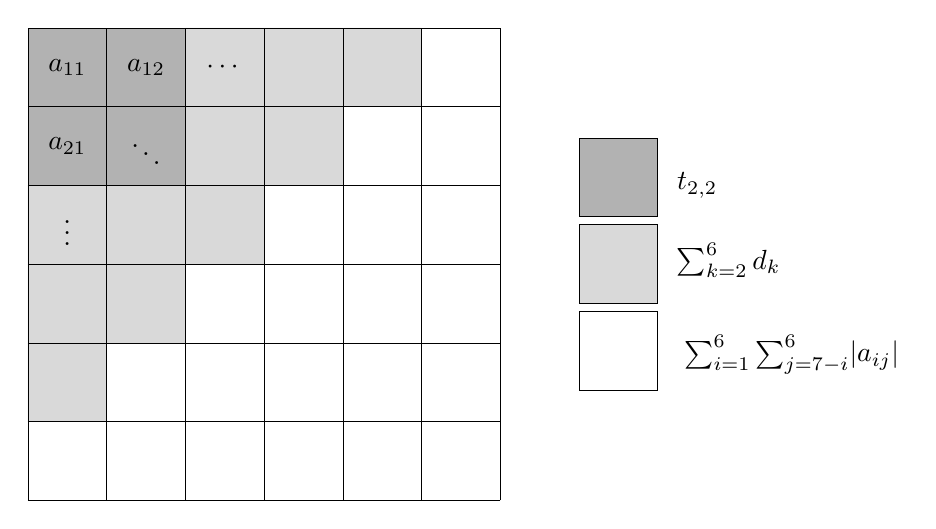
\begin{tikzpicture}
                \fill[color=black!30] (0,4) rectangle (2,6);
                \fill[color=black!15] (2,5) rectangle (5,6) (2,4) rectangle (4,5) (0,3) rectangle (3,4) (0,2) rectangle (2,3) (0,1) rectangle (1,2);
                \draw[step=1cm, black, very thin] (0, 0) grid (6, 6);

                \node at (0.5,5.5) {$a_{11}$};
                \node at (1.5,5.5) {$a_{12}$};
                \node at (0.5,4.5) {$a_{21}$};
                \node at (0.5,3.5) {$\vdots$};
                \node at (2.5,5.5) {$\cdots$};
                \node at (1.5,4.5) {$\ddots$};

                \filldraw[draw=black, fill=black!30] (7,3.6) rectangle (8,4.6);
                \draw(8.5,4) node{$t_{2,2}$};
                \filldraw[draw=black, fill=black!15] (7,2.5) rectangle (8,3.5);
                \draw(8.9,3.05) node{$\sum_{k=2}^6 d_k$};
                \draw (7,1.4) rectangle (8,2.4);
                \draw(9.7,1.85) node{$\sum_{i=1}^6 \sum_{j=7-i}^6 \abs{a_{ij}}$};
            \end{tikzpicture}
            \caption{$s_{6,6}$} \label{fig:1}
        \end{figure}
    \end{enumerate}
\end{solution}

\begin{exercise}
\label{ex:7}
    Assume that \( \sum_{i=1}^{\infty} a_i \) converges absolutely to \( A \), and \( \sum_{j=1}^{\infty} b_j \) converges absolutely to \( B \).
    \begin{enumerate}
        \item Show that the iterated sum \( \sum_{i=1}^{\infty} \sum_{j=1}^{\infty} \abs{a_i b_j} \) converges so that we may apply Theorem 2.8.1.

        \item Let \( s_{nn} = \sum_{i=1}^n \sum_{j=1}^n a_i b_j \), and prove that \( \lim_{n \to \infty} s_{nn} = AB \). Conclude that
        \[
            \sum_{i=1}^{\infty} \sum_{j=1}^{\infty} a_i b_j = \sum_{j=1}^{\infty} \sum_{i=1}^{\infty} a_i b_j = \sum_{k=2}^{\infty} d_k = AB,
        \]
        where, as before, \( d_k = a_1 b_{k-1} + a_2 b_{k-2} + \cdots + a_{k-1} b_1 \).
    \end{enumerate}
\end{exercise}

\begin{solution}
    \begin{enumerate}
        \item Let \( A' = \sum_{i=1}^{\infty} \abs{a_i} \) and \( B' = \sum_{j=1}^{\infty} \abs{b_j} \). Suppose \( i \in \N \) is fixed. Then
        \[
            \sum_{j=1}^n \abs{a_i b_j} = \abs{a_i} \sum_{j=1}^n \abs{b_j} \to \abs{a_i} B' \text{ as } n \to \infty.
        \]
        It follows that
        \[
            \sum_{i=1}^n \abs{a_i} B' = B' \sum_{i=1}^n \abs{a_i} \to A' B' \text{ as } n \to \infty,
        \]
        i.e.\
        \[
            \sum_{i=1}^{\infty} \sum_{j=1}^{\infty} \abs{a_i b_j} = A' B'.
        \]

        \item For each \( n \in \N \) we have
        \[
            s_{nn} = \sum_{i=1}^n \sum_{j=1}^n a_i b_j = \left( \sum_{i=1}^n a_i \right) \left( \sum_{j=1}^n b_j \right).
        \]
        The Algebraic Limit Theorem now implies that \( \lim_{n \to \infty} s_{nn} = AB \), and Theorem 2.8.1 then gives the desired result.
    \end{enumerate}
\end{solution}

\noindent \hrulefill

\noindent \hypertarget{ua}{\textcolor{blue}{[UA]} Abbott, S. (2015) \textit{Understanding Analysis.} 2\ts{nd} edition.}

\end{document}